\def\lecturenumber{08}
\documentclass[11pt,a4paper]{article}
\usepackage[T1]{fontenc}
\usepackage[utf8]{inputenc}
\usepackage{lmodern}
\usepackage[margin=19mm,top=21mm,bottom=21mm,headheight=15pt]{geometry}
\usepackage{amsmath,amssymb,booktabs,array,graphicx,microtype}
\usepackage[dvipsnames]{xcolor}
\usepackage{enumitem,fancyhdr,listings,tcolorbox}
\usepackage[colorlinks=true,linkcolor=MidnightBlue,urlcolor=MidnightBlue]{hyperref}
\definecolor{courseblue}{HTML}{164B69}
\definecolor{pale}{HTML}{F0F5F7}
\pagestyle{fancy}
\fancyhf{}
\fancyhead[L]{\small\sffamily\color{courseblue}VALIDATED COMPUTING}
\fancyhead[R]{\small\sffamily Lecture \lecturenumber}
\fancyfoot[L]{\footnotesize Expanded lecture notes \textbullet\ October 2026}
\fancyfoot[R]{\footnotesize\thepage\ / 6}
\renewcommand{\headrulewidth}{0.4pt}
\setlength{\parindent}{0pt}
\setlength{\parskip}{5.5pt plus 1pt}
\setlength{\emergencystretch}{1.5em}
\setlist[itemize]{leftmargin=1.5em,itemsep=3pt,topsep=3pt}
\setlist[enumerate]{leftmargin=1.7em,itemsep=5pt,topsep=4pt}
\lstset{language=Python,basicstyle=\small\ttfamily,keywordstyle=\color{courseblue}\bfseries,
 commentstyle=\color{OliveGreen},stringstyle=\color{BrickRed},showstringspaces=false,
 columns=fullflexible,keepspaces=true,frame=single,rulecolor=\color{black!18},
 backgroundcolor=\color{black!2},aboveskip=6pt,belowskip=6pt,breaklines=true,
 xleftmargin=5pt,xrightmargin=5pt,framesep=5pt}
\newcommand{\R}{\mathbb R}
\newcommand{\fl}{\operatorname{fl}}
\newcommand{\abs}[1]{\left|#1\right|}
\newcommand{\heading}[2]{\section*{\color{courseblue}#1}\vspace{-4pt}{\small\sffamily\color{black!65}#2}\par\vspace{3pt}}
\newcommand{\opening}[2]{{\Large\sffamily\bfseries\color{courseblue}Lecture \lecturenumber\quad #1\par}\vspace{5pt}{\small #2}\par}
\newtcolorbox{question}[1]{colback=pale,colframe=courseblue!55,boxrule=0.4pt,
 arc=1mm,left=7pt,right=7pt,top=4pt,bottom=4pt,title={#1},fonttitle=\bfseries\small,
 coltitle=courseblue,colbacktitle=pale}
\newcommand{\reading}[1]{{\footnotesize\textbf{Reading and notebook.} #1\par}}
\hypersetup{pdfauthor={Validated Computing course},pdfsubject={Expanded introductory lecture notes with questions and exercises}}

\hypersetup{pdftitle={Lecture 08: Automatic differentiation and derivative bounds}}
\begin{document}
\opening{Automatic differentiation and derivative bounds}{Prerequisites: product and chain rules; Lectures 05--07.\newline
Goal: propagate derivatives through a computation and identify the extra conditions needed for rigorous bounds.}
\heading{1. A derivative without a differencing step}{0--13 minutes: a familiar approximation and its two errors}
Lecture 07 needed an enclosure of the derivative over a whole interval.
Hand differentiation works for short expressions, but it becomes tedious
and error-prone as computations grow. Automatic differentiation (AD) applies
the same elementary differentiation rules while evaluating the expression.
It introduces no finite-difference step size. Its arithmetic still matters.

Start with $p(x)=x^3-2x$, for which $p'(1)=1$. A forward difference is
\[
 \frac{p(1+h)-p(1)}{h}=1+3h+h^2,\qquad h\ne0,
\]
in exact real arithmetic. Thus its truncation error is $3h+h^2$ for positive
$h$. Smaller $h$ reduces this error. On a machine, however, the numerator
subtracts nearby approximations, and division by a small $h$ amplifies their
arithmetic errors. Eventually even the stored value of $1+h$ may equal $1$.
\begin{lstlisting}
def polynomial(x):
    return x*x*x - 2*x

for exponent in [2, 5, 8, 11, 14, 16]:
    h = 10.0**(-exponent)
    estimate = (polynomial(1.0+h) - polynomial(1.0)) / h
    print(exponent, estimate, abs(estimate-1))
\end{lstlisting}

\begin{center}
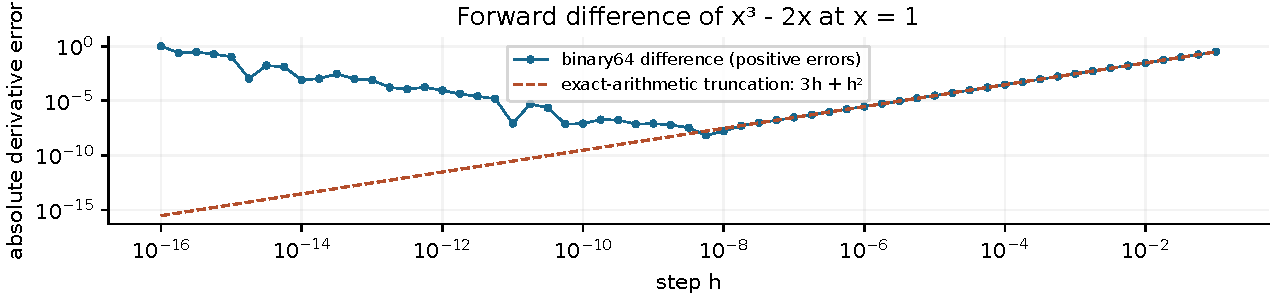
\includegraphics[width=0.85\linewidth]{figures/finite_difference_error.pdf}
\end{center}

The sampled curve illustrates the competition; its detailed shape depends
on the evaluation and arithmetic. The exact derivative and the algebraic
truncation formula supply the references. A small observed error is not an
interval certificate for derivatives on a neighborhood.

\begin{question}{Predict the failure at the smallest step}
If the stored value of $1+h$ equals $1$, what does the displayed quotient
become? Would computing $p'(1)$ accurately settle the range of $p'(x)$ on
$[1,2]$? Distinguish a point question from an interval question.
\end{question}

Finite differences remain useful when a function is accessible only through
evaluations. AD instead requires access to the operations defining the
computation and suitable differentiation rules for those operations.

\newpage
\heading{2. Carry a value and a tangent together}{13--29 minutes: derive the rules and trace a small computation}
Represent a quantity by a pair $(v,d)$. The first component is its value;
the second is its derivative with respect to the selected input direction.
For a scalar input $x$, start with $(x,1)$. A constant $c$ starts with $(c,0)$.
The second seed matters as much as the first: $(x,0)$ would track a direction
in which the input does not change.

The basic propagation rules follow directly from calculus:
\[
\begin{aligned}
 (v,d)+(w,e)&=(v+w,d+e),\\
 (v,d)-(w,e)&=(v-w,d-e),\\
 (v,d)(w,e)&=(vw,dw+ve),\\
 (v,d)^{-1}&=(1/v,-d/v^2),\qquad v\ne0.
\end{aligned}
\]
For a differentiable elementary function $g$, the rule is
$(v,d)\mapsto(g(v),g'(v)d)$. For example, exponentiation gives
$(e^v,e^vd)$ and sine gives $(\sin v,(\cos v)d)$.

\textbf{A useful algebraic interpretation.} Write the pair formally as
$v+d\varepsilon$ with $\varepsilon^2=0$. Multiplication then retains
$vw+(dw+ve)\varepsilon$. These are called dual numbers. The symbol
$\varepsilon$ is not a very small floating-point number: its square is zero
by an algebraic rule. There is no limiting process or numerical step size.

At $x=1$, evaluate $x^3-2x$ using the same intermediate quantities as the
original expression. Each row consumes only previously computed pairs.
\begin{center}
\begin{tabular}{llll}
\toprule
Quantity & Value & Tangent & Rule\\
\midrule
$x$ & $1$ & $1$ & input seed\\
$u=x\cdot x$ & $1$ & $1\cdot1+1\cdot1=2$ & product\\
$v=u\cdot x$ & $1$ & $2\cdot1+1\cdot1=3$ & product\\
$w=2x$ & $2$ & $0\cdot1+2\cdot1=2$ & constant and product\\
$v-w$ & $-1$ & $3-2=1$ & subtraction\\
\bottomrule
\end{tabular}
\end{center}

This calculation did not first construct the symbolic expression $3x^2-2$.
It propagated derivatives locally through the original evaluation. With exact
rational components, the point value and derivative in the table are exact.

\begin{question}{Derive a rule instead of memorizing it}
Differentiate the identity $v(1/v)=1$ to obtain the reciprocal tangent.
Where does the condition $v\ne0$ enter? If the input pair is $(x,2)$,
what quantity will the final tangent represent?
\end{question}

For one input direction, each arithmetic operation adds a bounded amount of
derivative work. This is \emph{forward mode}. The cost grows with the number
of directions requested; two variables will require two passes for a full
Jacobian in our straightforward implementation.

\newpage
\heading{3. Make the propagation rules visible in Python}{29--45 minutes: exact point arithmetic and the induction argument}
The following functions use pairs explicitly, so the product rule remains
visible. A class can later implement the same rules behind ordinary operators.
Constants must use zero tangents and arithmetic types appropriate to the
computation. Run the excerpts in this lecture in order.
\begin{lstlisting}
from fractions import Fraction

def add_pairs(left, right):
    return left[0] + right[0], left[1] + right[1]

def subtract_pairs(left, right):
    return left[0] - right[0], left[1] - right[1]

def multiply_pairs(left, right):
    value, tangent = left
    other_value, other_tangent = right
    product = value * other_value
    first_term = tangent * other_value
    second_term = value * other_tangent
    return product, first_term + second_term

def polynomial_pair(x):
    square = multiply_pairs(x, x)
    cube = multiply_pairs(square, x)
    two = (Fraction(2), Fraction(0))
    twice_x = multiply_pairs(two, x)
    return subtract_pairs(cube, twice_x)

result = polynomial_pair((Fraction(1), Fraction(1)))
assert result == (Fraction(-1), Fraction(1))
\end{lstlisting}

\textbf{Why the method works.} At input nodes and constant nodes, the seeds
are the correct values and derivatives. Assume both components are correct
for the operands of the next operation. Its calculus rule makes the two
new components correct as well. Induction through the finite expression
establishes the final value and derivative. Reusing an intermediate value
does not change this argument.

\textbf{What changes with floating-point components?} The same rules compute
approximations to the value and derivative. Products and sums in the tangent
can round or cancel, just as ordinary value computations can. AD removes
finite-difference truncation error; it does not remove arithmetic error.
It differentiates the smooth real expression represented by the operations,
not the discontinuous mapping caused by rounding every intermediate result.

\begin{question}{Separate three claims}
Which claim follows from the exact-rational assertion above? Which additional
work is needed for a floating-point result to be an enclosure? Why would
agreement with a finite-difference estimate be a diagnostic rather than a proof?
\end{question}

The explicit expression in \texttt{polynomial\_pair} is intentionally short.
Notebook 08 introduces a \texttt{Dual} class so longer expressions can retain
their original mathematical syntax while using these same propagation rules.

\newpage
\heading{4. Interval components enclose whole derivative ranges}{45--63 minutes: the same rules, with a stronger arithmetic contract}
Seed an input interval as $(X,[1,1])$. Suppose every component operation
preserves inclusion and every real operation is differentiable throughout
the relevant domain. Fix an arbitrary $x\in X$. The pair induction now shows
that each computed value component contains its real value at $x$, and each
tangent component contains its real derivative at $x$. Since $x$ was
arbitrary, the final components enclose both ranges over $X$.

For $x^3-2x$ on $[1,2]$, elementary interval propagation gives
\[
 (X,[1,1])^2=([1,4],[2,4]),\quad
 (X,[1,1])^3=([1,8],[3,12]).
\]
Subtracting the pair for $2x$ gives value enclosure $[-3,6]$ and derivative
enclosure $[1,10]$. The true value range is $[-1,4]$, while the derivative
range happens to be exact. Inclusion does not promise sharpness of either
component; repeated variables can lose dependence in both.

Here is an elementary-function example using Arb balls through
\texttt{python-flint}. It requires no course-package import.
\begin{lstlisting}
from flint import arb, ctx, fmpq

def exp_pair(x):
    value, tangent = x
    exponential = value.exp()
    return exponential, exponential * tangent

def sin_pair(x):
    value, tangent = x
    return value.sin(), value.cos() * tangent

with ctx.workprec(100):
    domain = arb(fmpq(-1, 4)).union(arb(fmpq(1, 4)))
    x = (domain, arb(1))
    value, tangent = multiply_pairs(exp_pair(x), sin_pair(x))
    if not value.is_finite() or not tangent.is_finite():
        raise ValueError("No finite pair of bounds")
    lower = tangent.mid().fmpq() - tangent.rad().fmpq()
    upper = tangent.mid().fmpq() + tangent.rad().fmpq()
    assert lower <= 1 <= upper  # Independent check at x = 0.
    assert lower > 0
\end{lstlisting}

The positive lower endpoint proves that $e^x\sin x$ is strictly increasing
on $[-1/4,1/4]$. Checking the known value $f'(0)=1$ alone would not establish
the all-input guarantee; the interval propagation argument supplies it.
Both elementary functions are smooth on any enlargement caused by the input ball.

\reading{API: \href{https://python-flint.readthedocs.io/en/latest/arb.html}{python-flint real-ball arithmetic}.
Exact rational midpoint/radius extraction follows Lecture 05.}

\newpage
\heading{5. A Jacobian is several directional derivatives}{63--77 minutes: seed one variable at a time}
For a map $F:\R^2\to\R^2$, the Jacobian has entries
$J_{ij}=\partial F_i/\partial x_j$: rows index outputs and columns index
inputs. If input tangents form a vector $s$, each propagated output tangent
is the derivative along that direction. Together the output tangents form
$J_F(x)s$. One pass supplies a column only when $s$ is the corresponding
coordinate direction.

Consider
\[
 F(x,y)=\begin{pmatrix}x^2+y^2-1\\x-y\end{pmatrix},\qquad
 J_F(x,y)=\begin{pmatrix}2x&2y\\1&-1\end{pmatrix}.
\]
Seed $(\dot x,\dot y)=(1,0)$ for the first column, then $(0,1)$ for the
second. At $(2,3)$, the columns are $(4,1)^T$ and $(6,-1)^T$.
\begin{lstlisting}
def system_pairs(x, y):
    x_squared = multiply_pairs(x, x)
    y_squared = multiply_pairs(y, y)
    total = add_pairs(x_squared, y_squared)
    one = (Fraction(1), Fraction(0))
    first = subtract_pairs(total, one)
    second = subtract_pairs(x, y)
    return first, second

first_pass = system_pairs((Fraction(2), Fraction(1)),
                          (Fraction(3), Fraction(0)))
second_pass = system_pairs((Fraction(2), Fraction(0)),
                           (Fraction(3), Fraction(1)))
jacobian = []
for row in range(2):
    jacobian.append([first_pass[row][1], second_pass[row][1]])
assert jacobian == [[4, 6], [1, -1]]
\end{lstlisting}

For a box $x\in[1,2]$, $y\in[3,4]$, interval components and the same seeds
give the matrix enclosure
\[
                 \begin{pmatrix}[2,4]&[6,8]\\{}[1,1]&[-1,-1]\end{pmatrix}.
\]
Every real Jacobian on the box lies entry by entry in this interval matrix.
The entries are generally correlated: arbitrary choices from all four
intervals need not describe a Jacobian at a single common input. Later
validated matrix operations must allow that possible overestimation.

\begin{question}{A seed determines the question}
At $(2,3)$, what output tangents result from seeding both inputs with one?
Why is the vector $(10,0)^T$ not the full Jacobian? Explain the input path
whose derivative it represents, and why two separate columns are needed.
\end{question}

The point $(2,3)$ need not solve $F(x,y)=0$ to evaluate its Jacobian.
Derivative computation and root certification are separate tasks. Lecture 10
will use a Jacobian enclosure as one ingredient in a local system certificate.

\newpage
\heading{6. Boundaries of the method and exercises}{77--90 minutes: audit a branch and select two exercises}
AD rules apply on differentiable domains. The point program
\texttt{x if x > 0 else -x} describes $|x|$. An interval crossing zero
contains both branches and a nondifferentiable point. Selecting the branch
at the midpoint cannot enclose a derivative over that interval. Even for a
smooth piecewise function, one must justify which branches are possible
and how their derivatives combine. The simple pair code performs no branch
analysis and must not be used to bypass these obligations.

Similarly, a reciprocal requires a denominator excluding zero. A very narrow
interval around zero does not supply that premise. General library calls,
such as arbitrary NumPy functions, also need compatible differentiation and
inclusion rules; accepting a pair or returning a ball is not itself a proof.

\begin{enumerate}
\item \textbf{Trace exact pairs.} Evaluate $p(x)=x^3-2x$ at $x=2$, first
with tangent $1$ and then with tangent $3$. Predict both final components
before running the functions. Explain why the value stays fixed while the
tangent changes.

\item \textbf{Derive and check a reciprocal.} Write a pair reciprocal for
exact rational components with nonzero value. Use it to differentiate
$(x+3)/(x+4)$ at $x=1$. Find an interval on which division would require
rejection in the bounded-interval arithmetic of this course.

\item \textbf{Dependency in a derivative.} Propagate the pair for $x^3-2x$
over $[-1,1]$ using ordinary two-operand interval multiplication throughout.
Compare the derivative bound with $3\operatorname{square}(X)-2$.
Why are different bounds possible although the derivative formulas agree
at each real input? Which one uses the one-variable square relation?

\item \textbf{Read the seeds.} For $H(x,y)=(x^2+xy,x-y)$, derive its
Jacobian by hand and using two pair passes. Give an interval matrix on
$[1,2]\times[3,4]$. If only the directional derivative along $(1,1)$ is
wanted, how many forward passes are needed?
\end{enumerate}

\textbf{Selected checks.} Exercise 1 gives $(4,10)$ and $(4,30)$.
Exercise 2 gives value $4/5$ and derivative $1/25$; a domain containing
$-4$ fails the denominator condition. Exercise 3 gives derivative enclosure
$[-5,1]$ from pair propagation, versus $[-2,1]$ from the sharp-square
formula; the latter is the true derivative range. Exercise 4:
$J_H=\left(\begin{smallmatrix}2x+y&x\\1&-1\end{smallmatrix}\right)$,
so an enclosure is
$\left(\begin{smallmatrix}[5,8]&[1,2]\\{}[1,1]&[-1,-1]\end{smallmatrix}\right)$.
One pass suffices for one specified direction.

\begin{question}{Exit ticket: what error or premise remains?}
Compare a finite difference, floating-point AD, and interval AD. Identify
truncation error, arithmetic error, dependency overestimation, and domain
assumptions where they apply. Which method can supply the derivative
enclosure required by the mean-value theorem in Lecture 07?
\end{question}

\reading{Companion: \texttt{notebooks/08\_automatic\_differentiation.ipynb}
and Lab 08. Tucker (2011), \S4.1, pp.~60--64. Higher derivatives in
\S\S4.2--4.3 are optional extensions. Next: scalar root certificates.}
\end{document}
